\label{desenvolvimento_processamento}

Nesta seção é descrito o detalhamento da solução do módulo de interface/processamento, resultante das duas primeiras fases,
e o seu projeto e construção, resultante da Fase 03.
Além disso, a visão da solução e da arquitetura estão documentadas nos Apêndices \ref{documento_visao} e \ref{documento_arquitetura}, respectivamente.

\subsection{Detalhamento da Solução} \label{software:detalhamento_solucao}

A solução completa definida nas Fases 01 e 02 pode ser vista no \href{https://drive.google.com/file/d/0B5InkGKx6O-MR1B3eVYzZFpjQ3c/view?usp=sharing}{Relatório 1}.

A Figura \ref{fig:arquitetura_solucao} apresenta a solução proposta como um todo e nela podemos destacar a atuação da
frente de interface/processamento nos seguintes subsistemas de software:

\begin{itemize}
 \item \textbf{Interface de comunicação entre o usuário e a bancada, realizada por meio da aplicação web;}
      \subitem Na aplicação web o usuário poderá controlar a bancada, iniciando um ensaio com os quesitos definido por ele,
	       e visualizar os resultados do ensaio por meio de gráficos.
 \item \textbf{Servidor de Controle para intermediar a comunicação da aplicação web com o sistema de controle eletrônico, hospedado na \textit{Raspberry}.}
      \subitem Este servidor provê serviços RESTFul (API REST) como a interface de comunicação para a aplicação web. Neste servidor estão as 
	       rotinas de comunicação com o sistema de controle eletrônico, que realizam a inserção de dados de comando e recupera os dados 
	       dos sensores via comunicação serial.
\end{itemize}

A interação entre esses dois subsistemas que compõem o módulo de interface/processamento funcionará da seguinte forma
(o protocolo de comunicação definido será apresentado na subseção \ref{software:protocolo}):

\begin{enumerate}
 \item O usuário cadastrado autentica-se no sistema (caso o usuário não seja cadastrado basta ele se cadastrar);
 \item O usuário monta um ensaio com seus respectivos \textit{jobs} (o conceito de \textit{job} é apresentado na subseção \ref{software:app_web});
 \item O usuário confere os sensores ativos identificados pelo sistema e inicia o experimento;
    \subitem O usuário tem a possibilidade de atualizar os sensores ativos, caso perceba erro na leitura dos sensores;
    \subitem Quando o usuário solicita a identificação dos sensores ativos, a aplicação web envia uma requisição
         de identificação dos sensores ativos ao Servidor de Controle, seguindo o protocolo definido.
 \item A aplicação web envia uma requisição ao Servidor de Controle informando os dados dos \textit{jobs} 
        e sinalizando que o experimento começou;
       \subitem A cada novo \textit{job} que deve começar (mudança de frequência da mesa) a aplicação web envia uma requisição
       de solicitação de alteração de frequência da mesa, seguindo o protocolo definido.
 \item O Servidor de Controle, então, envia uma mensagem ao sistema de controle (via rotinas de comunicação,
       que serão apresentadas na subseção \ref{software:rotinas}) informando o início do experimento e a frequência
       desejada (frequência do \textit{job} corrente) e inicia uma \textit{thread} para a coleta dos dados lidos dos sensores;
 \item Quando o último \textit{job} chegar ao fim, a aplicação web envia uma requisição ao Servidor de Controle informando
       que o ensaio acabou, o que significa que o sistema de controle não precisa mais coletar dados dos sensores;
 \item Quando o Servidor de Controle recebe essa requisição, este envia uma mensagem ao sistema de controle (via rotinas de comunicação)
       informando a parada da coleta dos dados dos sensores, seguindo o protocolo definido;
 \item A aplicação web informa ao usuário que está aguardando o término da coleta e processamento dos dados enquanto o Servidor de
       Controle coleta o restante dos dados dos sensores e a aplicação web processa os dados coletados;
 \item Quando todos os dados amostrados forem coletados, o Servidor de Controle repassa esses dados para a aplicação web e
       destes serão derivados os outros dados necessários para a aplicação, seguindo 
       o método apresentado na seção \ref{software:processamento}. O processamento dos dados aqui mencionado se refere aos cálculos da frequência,
       velocidade e amplitude a partir da aceleração fornecida pelos sensores;
 \item Com todos os dados calculados, a aplicação web monta os gráficos e apresenta os resultados do ensaio ao usuário.
\end{enumerate}


Nas próximas subseções são detalhados os dois subsistemas propostos como solução para o módulo de interface de processamento.


\subsection{Projeto e Construção}

  Nesta subseção é apresentado o projeto e construção dos subsistemas propostos na Subseção \ref{software:detalhamento_solucao},
  bem como as mudanças realizadas no que foi proposto.

\subsubsection{\textbf{Interface de comunicação com o usuário - Aplicação Web}} \label{software:app_web}
    
    Como  apresentado no \href{https://drive.google.com/file/d/0B5InkGKx6O-MR1B3eVYzZFpjQ3c/view?usp=sharing}{Relatório 1},
    a aplicação web servirá para o usuário controlar a bancada e visualizar os resultados dos ensaios, contando com os seguintes requisitos
    funcionais (conforme \textit{backlog} apresentado no \href{https://drive.google.com/file/d/0B5InkGKx6O-MR1B3eVYzZFpjQ3c/view?usp=sharing}{Relatório 1})
    para atender as necessidades do usuário (vide Apêndice \ref{documento_visao} para as necessidades do usuário):
    
    \begin{itemize}
      \item \textbf{Cadastro de usuários;}
	 \subitem Os usuários da bancada (alunos, professores e técnicos) devem ser cadastrados no sistema para utilizar a bancada.
      \item \textbf{Acesso ao sistema;}
	 \subitem Os usuários cadastrados devem ter acesso ao sistema para realizar ensaios.
      \item \textbf{Início do ensaio;}
	 \subitem Deve ser possível a criação de um ensaio específico pelo usuário, informando a frequência e tempo de ensaio desejados.
      \item \textbf{Visualização dos ensaios realizados;}
	 \subitem Os ensaios de um usuário devem ser mantidos no sistema, para que o usuário possa visualizar os resultados de um ensaio
		  já realizado quando quiser;
      \item \textbf{Visualização dos resultados do ensaio;}
	 \subitem Os resultados do ensaio realizado deve ser apresentado em formas de gráficos para facilitar a interpretação dos resultados.
    \end{itemize}
     
    Para o requisito "Início do ensaio" o usuário necessita poder criar um ensaio com diferentes frequências a serem testadas no mesmo ensaio.
    Para implementar este requisito foi realizada um abstração do ensaio como um conjunto de \textit{jobs}.
    Um \textit{job} é uma parte do ensaio com uma frequência e tempo fixo. Exemplificando, caso o usuário queira um ensaio que começa com uma
    frequência de 50Hz por 10s e depois mude para 80Hz e permaneça por mais 15s, basta criar um ensaio com dois \textit{jobs}, onde o primeiro
    \textit{job} teria frequência igual a 50Hz e tempo de 10s e o segundo teria frequência igual a 80Hz e tempo de 15s.
    
    Com o intuito de visualizar a solução Web foi desenhado um protótipo de alta fidelidade da aplicação Web. 
    As telas podem ser vistas no \href{https://drive.google.com/file/d/0B5InkGKx6O-MR1B3eVYzZFpjQ3c/view?usp=sharing}{Relatório 1}.
    
    Como definido no \href{https://drive.google.com/file/d/0B5InkGKx6O-MR1B3eVYzZFpjQ3c/view?usp=sharing}{Relatório 1},
    a aplicação web foi desenvolvida utilizando o \textit{framework} Django (em linguagem Python) de acordo com as justificativas
    apresentadas também no Relatório 1. 

\subsubsection{\textbf{Interface de comunicação com o sistema de controle - Servidor de Controle}}
   
   Esta subseção apresenta o projeto e construção do servidor RESTFul que será hospedado na \textit{Raspberry} para intermediar a comunicação
   com o sistema de controle. Este servidor é chamado aqui de Servidor de Controle.
  
\subsubsubsection*{\textbf{Mudanças - Aspectos gerais}}
    
Ao final do primeiro ponto de controle, a frente de interface/processamento, em suma, havia estabelecido os seguintes requisitos não-funcionais para o \textbf{software}:

\begin{itemize}
    \item Aplicação \textit{Web} para uso por parte do usuário, sendo esta desenvolvida com o \textit{framework} Django (que utiliza linguagem de programação \textit{Python}) juntamente com o SGBD (Sistema Gerenciador de Banco de Dados) \textit{MySQL}.
    \item Aplicação \textit{REST} para recebimento de comandos e fornecimento de dados para a Aplicação \textit{Web}, sendo esta desenvolvida com o Django \textit{REST} \textit{Framework} juntamente com a base de dados \textit{SQLite}.
    \item Rotinas de comunicação em linguagem C para escrita e leitura de dados na porta serial existente na \textit{Raspberry}.
\end{itemize}


Durante a execução do projeto, constatou-se que não haveria mais necessidade de uso da linguagem C, aspecto que será melhor detalhado na
próxima subseção, sobre as mudanças no projeto das rotinas de comunicações.
Outro aspecto alterado foi a base de dados utilizada pelo \textit{REST}, optando-se pelo uso do \textit{MySQL} ao invés do \textit{SQLite}.

O SGBD \textit{MySQL} foi também adotado para a aplicação \textit{REST} pelos seguintes motivos:

\begin{itemize}
  \item É mais performático que o \textit{SQLite}.
  \item Não há travamentos da base de dados devido às operações, o que possibilita a concorrência no uso do banco de dados.
  \item Favorece a escalabilidade da solução.
\end{itemize}

\subsubsubsection*{\textbf{Arquitetura das Rotinas de Comunicação e Parser}} \label{software:rotinas}

Para realização das rotinas de comunicação e parser, a equipe de software contou com um simulador. O simulador, construído pela frente de eletroeletrônica, 
consiste em um \textit{Arduino} que simula o comportamento da entrada e saída de dados que o sistema da \textit{Raspberry} terá de comunicar. Com isso 
então, foi possível realizar o desenvolvimento das rotinas de comunicação em \textit{Python}, bem como iniciar também o \textit{Parser}.

O \textit{Parser} foi construído utilizando a base de dados que o próprio \textit{Django} oferece, que no caso é o \textit{SQLITE3}, foi simulado uma 
entrada de uma \textit{String} seguindo o protocolo de comunicação e em seguida essa \textit{String} é tratada para que seja guardada no banco de dados 
da aplicação local. O primeiro passo consiste em conectar ao banco de dados, e em seguida realizar o tratamento dos dados em uma lista de forma a 
averiguar se os dados estão corretos de acordo com a entrada de elementos das tabelas no banco de dados. O próximo passo então insere os dados da lista 
no banco de dados, usando o método \textit{inserting acceleration} e assim por diante para os outros dados.

É importante ressaltar que o processamento está planejado para o ponto de controle 3, que utilizará essa base de dados local para realizar os cálculos 
e então inserir os dados de acordo com as tabelas de velocidade, amplitude e frequência, que serão utilizados pela aplicação web.

Com relação às rotinas de entrada e saída de dados, foi utilizado o \textit{Arduino} para fins de teste de comunicação. A frente de eletroeletrônica 
desenvolveu uma rotina que é executada no \textit{Arduino} que conseguia simular a entrada e saída de dados com o comportamento similar ao esperado. 
Então utilizado a biblioteca serial que é padrão em \textit{Python}, foi possível construir métodos abstraindo o controle da comunicação serial em baixo
nível para um alto nível, e conectá-los as rotinas que guardarão os dados, no caso o \textit{Parser}.

Para comunicação com a malha fechada de controle do sistema, foi desenvolvido o \textit{Pyserial}. Uma classe que abstrai os principais métodos da 
biblioteca padrão do \textit{Python} chamada serial. Com essa biblioteca foi possível inicializar os valores como \textit{BAUDRATE} (Taxa de transmissão),
\textit{Timeout} e a porta serial de entrada e saída dos dados. A classe também conta com um método simples que acumula os resultados de leitura da porta 
serial em uma grande lista que será utilizada pelo \textit{Parser} para o tratamento dos dados resultantes para que eles possam ser guardados no banco de 
dados. A classe também conta com um tratamento de exceções para evitar que as exceções subam em nível de usuário.

O \textit{RoutinesUtil}, é uma classe que faz parte da solução em \textit{Django} no pacote de classes e ele é responsável por definir o comportamento 
da rotina. Nesta classe são definidas as rotinas de leitura de dados resultantes, dos sensores ativos e da escrita de controle do sistema. Ela utiliza 
as classes \textit{Pyserial} e \textit{Parser} para abrir a porta serial, ler os dados, fechar a porta serial e gravar no banco de dados da aplicação do 
servidor, que mandará para aplicação Web.

A integração entre eletroeletrônica e software vem com as rotinas que irão se comunicar com a malha fechada de controle do sistema e com a 
\textit{Raspberry} da aplicação, responsáveis por armazenar os resultados e processá-las para a aplicação web. Na imagem abaixo você poderá verificar 
o diagrama de classes parcial das rotinas de comunicação em integração com o \textit{Django} da \textit{Raspberry} e seus respectivos métodos.

\begin{figure}[H]
\centering
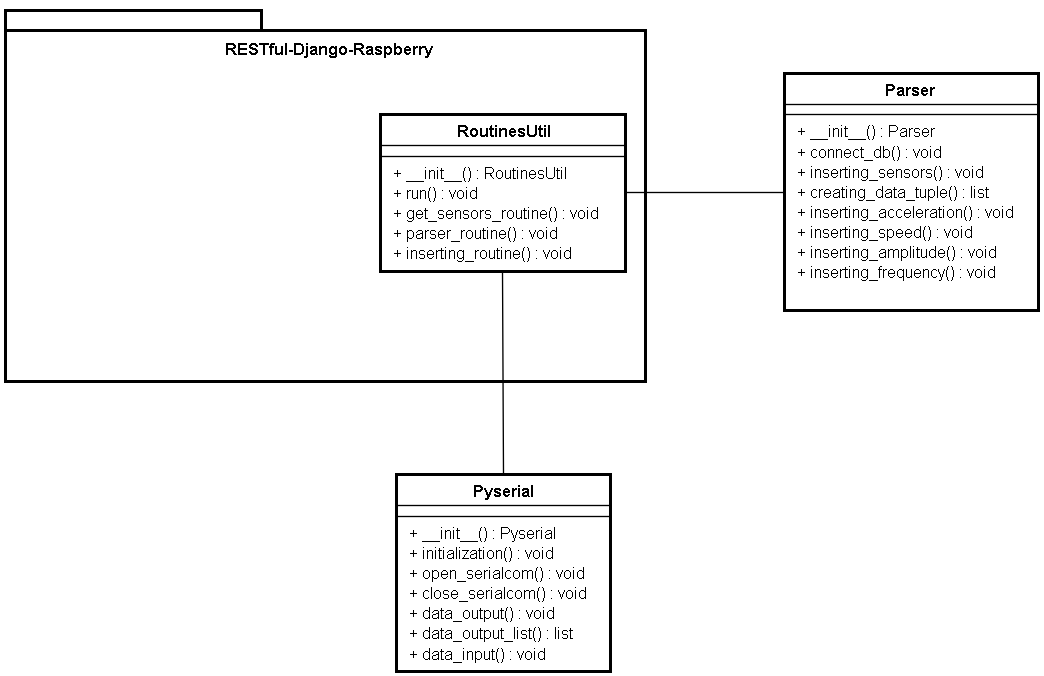
\includegraphics[keepaspectratio=true,scale=0.65]{figuras/uml_routines_parser.png}
\label{fig:uml_routines_parser}
\caption{Diagrama de Classes Parcial das Rotinas de Comunicação e Parser, integrados ao \textit{Django} - Fonte: Autor}
\end{figure}


\subsubsubsection*{\textbf{Mudanças - Rotinas de Comunicação}}

A camada de software na aplicação Web foi desenvolvida em \textit{Python}, bem como a camada de servidor de comunicação com a aplicação na 
\textit{Raspberry}. Como foi relatado, os membros do grupo naquele momento haviam chegado ao consenso de utilizar a linguagem C para integrar 
com \textit{Python}, que seria utilizado nas rotinas de comunicação entre \textit{Raspberry} e os microcontroladores da aplicação de baixo nível.

Durante o desenvolvimento das rotinas de comunicação, percebeu-se que não havia necessidade de que as mesmas fossem desenvolvidas 
usando tal linguagem, considerando que a linguagem C é uma linguagem de baixo nível normalmente utilizada para ter um maior controle sobre o 
hardware, o que não é o caso do projeto. Levando em consideração este fato, foi levantada a hipótese de utilização do módulo de comunicação serial que o próprio 
\textit{Python} oferece, e para isso foi realizado uma lista de prós e contras acerca da linguagem no desenvolvimento das rotinas de comunicação.

Utilizando a linguagem C para o desenvolvimento das rotinas de comunicação possui as seguintes vantagens:

\begin{itemize}
    \item A linguagem C é uma linguagem de baixo nível, ou seja, oferece um maior controle do hardware, e fornece a possibilidade de manipulações com \textit{bytes} em uma maior flexibilidade do que com as demais linguagens, exceto a linguagem \textit{ASSEMBLY}.
    \item Com a linguagem C é possível desenvolver o sistema de forma a se proteger contra falhas críticas, impedindo de repassar erros de baixo nível para a camada de alto nível.
    \item A linguagem C realiza processamentos mais velozes em comparação com as outras linguagens como \textit{Python}, dentre outras, se tornando uma excelente ferramenta para manipulação de \textit{bytes}.
\end{itemize}

Desvantagens da utilização da linguagem C para o desenvolvimento das rotinas de comunicação:

\begin{itemize}
    \item Por ser uma linguagem de baixo nível com uma alta tipagem, o trabalho de desenvolver uma rotina de comunicação serial usando recursos da camada de hardware se tornam bastante complexos.
    \item Na arquitetura proposta no primeiro ponto de controle, as rotinas de escrita e leitura de dados funcionariam da seguinte maneira: a escrita iria ler um arquivo, em seguida iria apagá-lo e então, enviaria este dado para o sistema de controle; no sistema de leitura, seria aberta a porta seria para leitura dos \textit{bytes}, que seriam decodificados e transcritos num arquivo para serem lidos por uma rotina \textit{Python} para escrever no banco de dados. Ou seja, a integração possui uma alta complexidade.
    \item Apesar da linguagem C ser mais rápida que \textit{Python}, não existe necessidade das rotinas serem desenvolvidas em tal linguagem, pois a diferença de velocidade de escrita e leitura para comunicação serial é bem mínima levando em consideração ao que \textit{Python} também faz.
\end{itemize}

Vantagens em utilizar \textit{Python} para o desenvolvimento das rotinas de comunicação:

\begin{itemize}
    \item Python possui uma baixa tipagem.
    \item Possui uma biblioteca de comunicação serial que realiza a abstração do jeito que o desenvolvedor quiser (seja controlar em baixo nível, ou em alto nível com uma abstração do controle).
    \item Fácil integração com \textit{RESTful} do \textit{Django} que é realizado em \textit{Python}.
    \item Elimina necessidade de escrever e ler em arquivos, pois os métodos podem ser carregados pelo \textit{REST} diretamente, assim o \textit{REST} terá o controle total da comunicação.
    \item Não existe necessidade de manipular leitura e escrita de bytes, devida a abstração da biblioteca.
    \item \textit{Python} é uma linguagem melhor para manipulação de dados, e permitirá a escrita dos dados recebidos diretamente no banco de dados do servidor da \textit{Raspberry}, que a aplicação irá utilizar.
\end{itemize}

Desvantagens da linguagem \textit{Python} para o desenvolvimento das rotinas de comunicação:

\begin{itemize}
    \item \textit{Python} é uma linguagem interpretada e mais lenta em comparação à linguagem C.
    \item Não fornece um controle maior em comparação às linguagens de baixo nível.
\end{itemize}

Com a nova mudança então, a única linguagem de programação que está sendo utilizada neste projeto é a linguagem \textit{Python}, e em virtude 
desta mudança, a arquitetura mudou um pouco agora, sendo nesse novo estilo.

\begin{figure}[H]
\centering
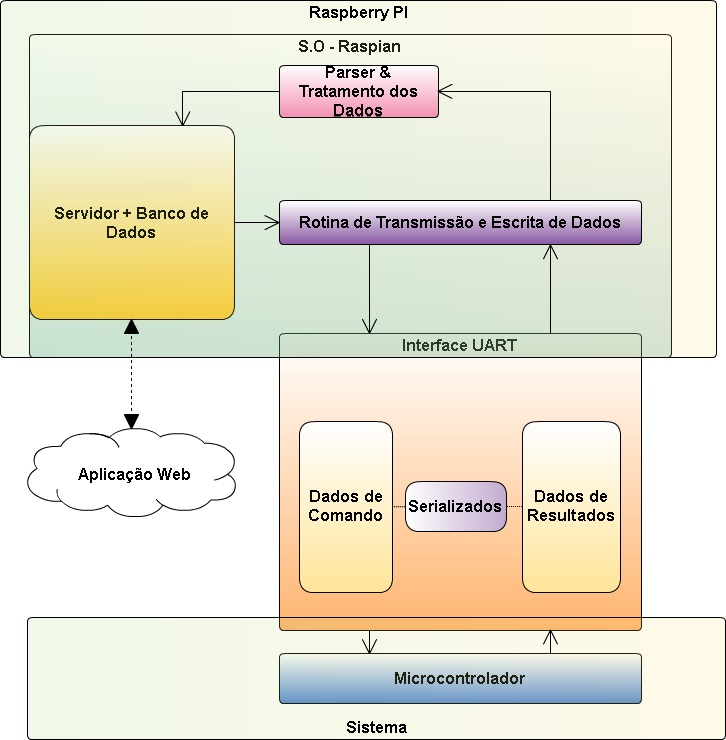
\includegraphics[keepaspectratio=true,scale=0.7]{figuras/nova_arquitetura.png}
\label{fig:nova_arquitetura}
\caption{Nova arquitetura com a mudança da linguagem implementada - Fonte: Autor}
\end{figure}

\subsubsection*{\textbf{Protocolo de Comunicação}} \label{software:protocolo}

As rotinas de comunicação são as pontes pelas quais os componentes de software do servidor que estará rodando na \textit{Raspberry} irão se
comunicar com os componentes eletroeletrônicos do sistema de controle e, consequentemente, com o resto do sistema. 
Para que a comunicação seja estabelecida é necessário estabelecer um padrão de comunicação de acordo com ambas as frentes, de forma que a comunicação 
ocorra com sucesso e sem surpresas. Foi definido então um protocolo de comunicação que deve ser respeitado pela frente de software e
eletrônica durante a transmissão de dados via serial.

Com a mudança da arquitetura ficou mais simples a integração das rotinas de comunicação e de escrita (com o parser dos dados) com o
servidor, o que nos permitiu formalizar um protocolo bem simples para a comunicação entre o sistema de controle e o sistema da aplicação.

O protocolo de comunicação é dividido em duas partes: o protocolo de controle e o protocolo de resposta, que são apresentados abaixo.

\begin{itemize}
    \item \textbf{Protocolo de Controle}
    \begin{itemize}
        \item É definido por \textit{flags} que permitirão que o sistema realize ações pré-definidas.
    \end{itemize}
    \item \textbf{Protocolo de Resposta}
    \begin{itemize}
        \item É definida a \textit{STRING} de resposta que o sistema de controle enviará para a camada de alto nível, no caso a \textit{Raspberry}, via 
        comunicação serial.
    \end{itemize}
\end{itemize}

\begin{figure}[H]
\centering
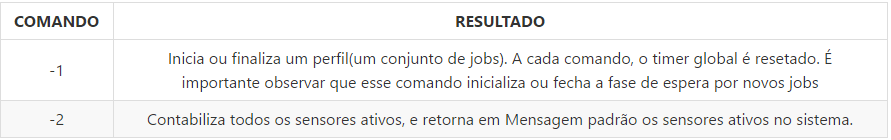
\includegraphics[keepaspectratio=true,scale=0.7]{figuras/protocolo_controle.png}
\label{fig:protocolo_controle}
\caption{Protocolo de Controle com \textit{flags} já definidas - Fonte: Autor}
\end{figure}

\begin{figure}[H]
\centering
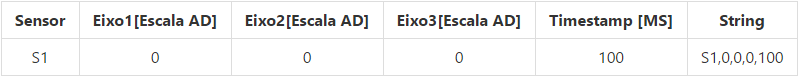
\includegraphics[keepaspectratio=true,scale=0.8]{figuras/protocolo_string.png}
\label{fig:protocolo_string}
\caption{Protocolo de Resposta e o formato da String que chegará ao sistema - Fonte: Autor}
\end{figure}

Com esse padrão definido, o usuário definirá um determinado número de \textit{jobs} (cada \textit{job} representa uma frequência com uma duração de tempo, 
e um conjunto de \textit{jobs} define um ensaio) que serão executados ao longo do ensaio. Ao executar o ensaio, os resultados dos sensores irão ser 
repassados na escala entre 0 a 1024 em AD (\textit{Analogic Digital}), sendo 0AD igual a 0G e 1024AD igual a 16G. Para determinar a aceleração a 
partir dessa escala basta utilizar uma regra de três simples. Por fim, esses dados passarão pelo processamento para serem persistidos no
banco de dados da \textit{Raspberry}.

Um dos objetivos ao obter a \textit{timestamp} a qual foi obtido o resultado pelo sensor é a necessidade de identificar e mapear os
\textit{jobs} de acordo com o ensaio, para ordenar e saber quais dados pertencem a quais \textit{jobs}.

A Figura \ref{fig:diagrama_sequencia_pc2} mostra um diagrama de sequência que apresenta a interação entre usuário, a aplicação web e o servidor da \textit{raspberry},
ilustrando como é tratado o \textit{input} e o \textit{output} do sistema como um todo entre os componentes de software e de eletrônica.

\begin{figure}[H]
\label{fig:diagrama_sequencia_pc2}
\centering
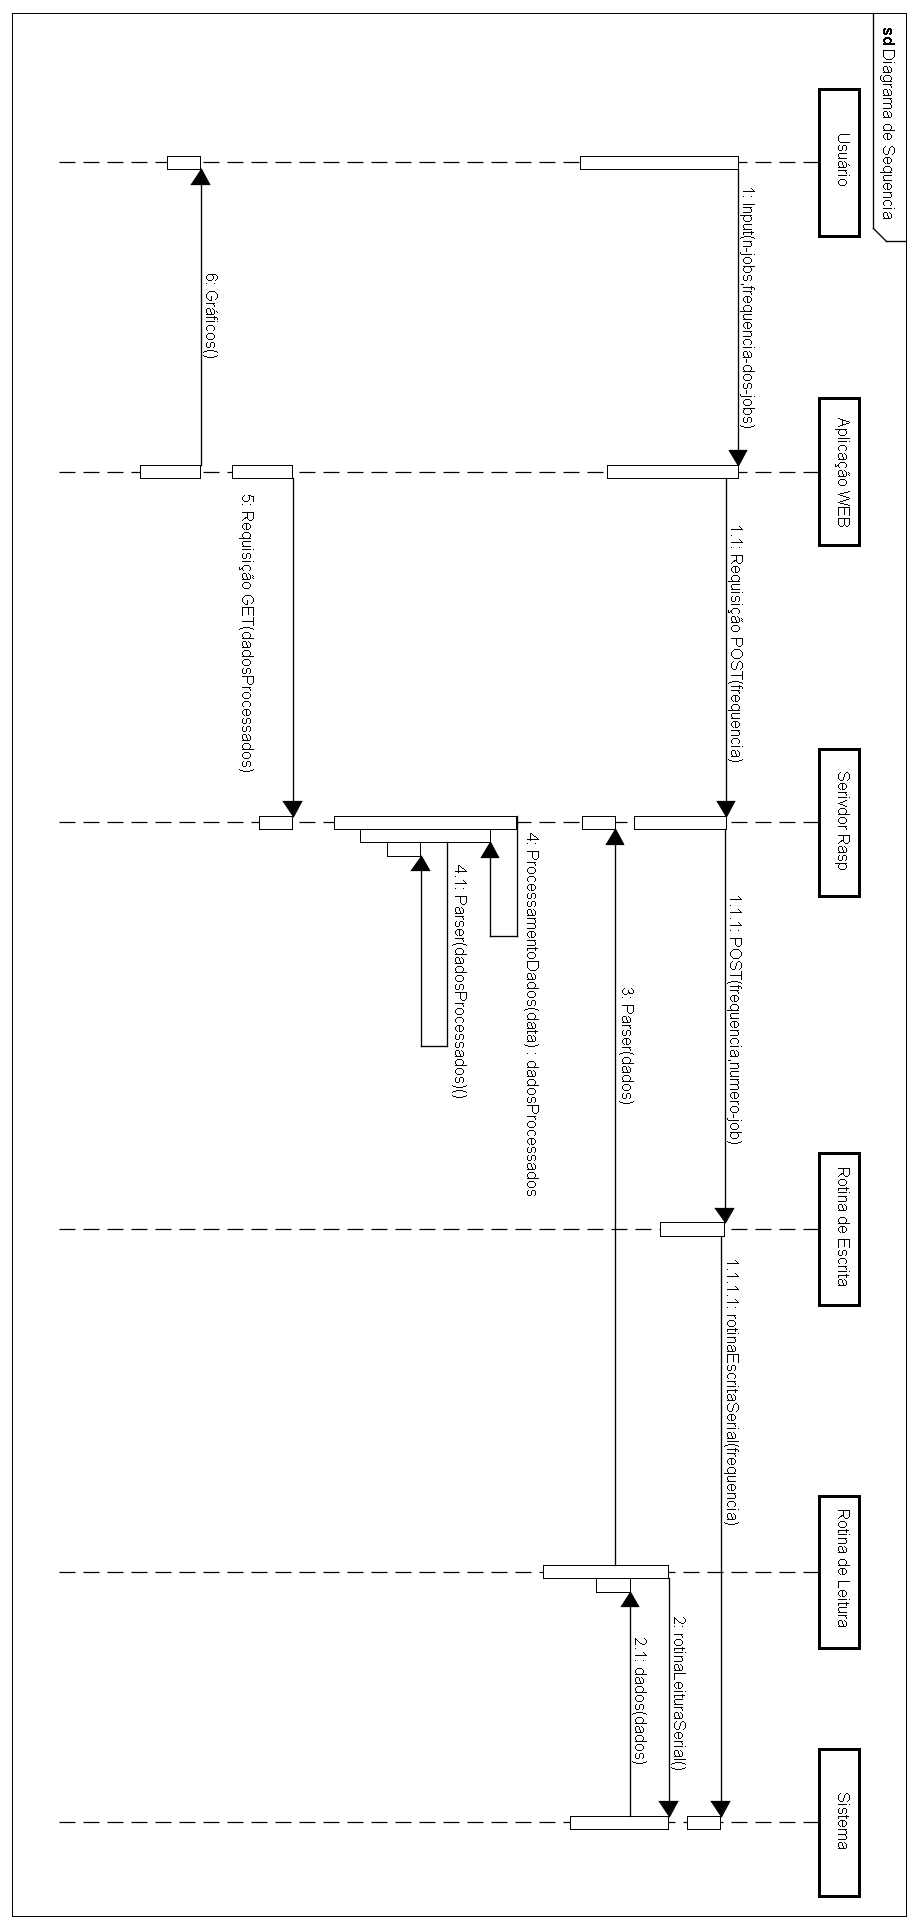
\includegraphics[keepaspectratio=true,scale=0.5]{figuras/diagrama_sequencia_pc2.png}
\caption{Diagrama de sequência - Fonte: Autor}
\end{figure}

\subsubsection*{\textbf{Processamento dos Dados}} \label{software:processamento}

Como mencionado, o processamento dos dados se refere ao cálculo da frequência, velocidade e amplitude a partir dos dados de aceleração
coletados dos sensores. Como os dados que se tem são coordenadas de aceleração por tempo, é preciso recorrer a integração numérica para 
cálcular esses dados, pois a velocidade (v(t)) é a integral da aceleração (a(t)) e o deslocamento (s(t)) é a integral da velocidade, como 
ilustram as fórmulas abaixo. A curva do deslocamento, neste caso, representa a amplitude (A) ao longo do tempo, pois o deslocamento calculado
da mesa, a partir dos dados dos sensores, representa o quanto a mesa subiu ou desceu (pois a mesa se move apenas no eixo Y).

$$ v(t) = \int_{}^{} a(t) dt$$
$$ A(t) = s(t) = \int_{}^{} v(t) dt$$

\subsubsubsection*{\textbf{Métodos numéricos analisados}}

A integral é uma das mais importantes ferramentas matemáticas e que aparece com frequência na solução de problemas e no cálculo de grandezas 
na engenharia e na ciência \cite{metodos_numericos}.

Na engenharia, há situações que envolvem dados experimentais ou de teste, nos quais uma grandeza física a ser determinada pode ser expressa 
como a integral de outras grandezas medidas. Assim, é válido ressaltar que o integrando pode ser uma função analítica ou um conjunto de pontos
discretos (dados tabulados).

Quando se tem um integrando expresso de forma que a integral pode ser facilmente calculada, pode-se obter analiticamente o valor da integral 
definida. A integração numérica faz-se necessária quando a integração analítica é difícil, ou mesmo impossível, e quando o integrando é fornecido
como um conjunto discreto de pontos \cite{metodos_numericos}.

Este é o caso da Bancada de Vibrações Mecânicas que está sendo construída neste projeto. Os dados que se tem são o retorno da leitura dos sensores 
e assim, o integrando é fornecido como um conjunto de pontos.

A análise numérica de uma integral caracteriza-se por estimar o número correspondente à integral de uma função entre os limites [a, b]. 
Caso seja utilizado apenas os pontos finais do intervalo, pode ser que o resultado fornecido não seja suficientemente preciso, especialmente se
o intervalo for significativamente grande ou se o integrando variar significativamente ao longo do intervalo. Dessa maneira, uma maior precisão 
pode ser obtida com o uso de um método composto, no qual o intervalo [a, b] é dividido em subintervalos menores. Assim, calcula-se a integral ao
longo de cada subintervalo e os resultados são somados para fornecer a integral completa.

É importante ressaltar que existem vários métodos disponíveis para o cálculo numérico de integrais. Esses métodos podem ser divididos em abertos 
e fechados. Os métodos de integração fechados consideram os pontos finais do intervalo e o integrando propriamente dito na fórmula que estima o
valor da integral. Já nos métodos de integração abertos, o intervalo de integração se estende além do limite especificado pelos pontos finais 
\cite{metodos_numericos}.

Devido à variedade de métodos, os principais foram analisados e verificou-se sua aplicação no âmbito do projeto. Os métodos considerados foram: 
Trapezoidal Composto, Métodos de Simpson e Quadratura de Gauss.

No {\textbf{Método Trapezoidal Composto}} a integral, ao longo do intervalo [a, b], pode ser avaliada de forma mais precisa com a subdivisão do 
intervalo, a avaliação da integral em cada um dos subintervalos e a soma dos resultados. A imagem a seguir ilustra a expansão genérica para a 
integração numérica por trapézios.

\begin{figure}[H]
\centering
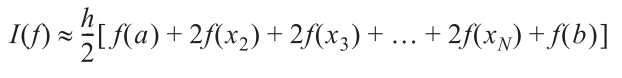
\includegraphics[keepaspectratio=true,scale=0.52]	{figuras/metodo_trapezoidal.png}
\label{fig:metodo_trapezoidal}
\caption{Integração numérica por Trapézios Acumulados - Fonte: \citeonline{metodos_numericos}}
\end{figure}

É importante notar que a fórmula do método trapezoidal composto se aplica precisamente para os casos onde os subintervalos têm uma largura h
idêntica. Outro aspecto interessante no uso desse método é que a precisão da resposta pode melhorar a partir da utilização de mais subintervalos.

O método trapezoidal aproxima o integrando por uma linha reta. De fato, seria melhor a aproximação por meio da representação do integrando 
como uma função não-linear e de fácil integração.

Há um grupo de métodos dotados desta característica, denominados \textbf{Métodos de Simpson}, utilizando polinômios quadráticos (método de
Simpson 1/3) e polinômios cúbicos, no caso do método de Simpson 3/8.

Os métodos de Simpson possuem restrições mais severas para uso. No caso do método de Simpson 1/3 composto, os subintervalos devem ser 
igualmente espaçados e o número de subintervalos no intervalo [a, b] deve ser um número necessariamente par. Com relação ao método de Simpson 
3/8 composto, além do espaçamento igual na identificação dos subintervalos, tem-se que o número de subintervalos no intervalo [a, b] deve ser 
divisível por 3.

Por fim, na \textbf{Quadratura de Gauss}, a integral também é avaliada utilizando a soma ponderada dos valores da função em pontos distintos 
ao longo do intervalo [a, b]. Nessa abordagem, são utilizados os pontos de Gauss, que, por sua vez, não são igualmente espaçados e não incluem 
os pontos finais.

Para o projeto da Bancada de Vibrações, optou-se pelo uso do método dos trapézios acumulados (método trapezoidal composto). A frente de 
controle projetou uma leitura dos dados dos sensores que garantirá intervalos de tempo igualmente espaçados, já favorecendo a aplicação de 
tal método. Outro aspecto interessante é que não será necessário controlar se o número de subintervalos é par ou se é divisível por três. 
O método dos trapézios se aplica independentemente deste aspecto.

Outro aspecto que deve ser notado é que como a massa de dados coletada a partir da leitura das medições feitas pelos sensores é grande, a
precisão do método será ainda maior.

Para implementação do método dos trapézios, por meio de pesquisa, foi encontrada a Biblioteca \textit{SciPy}, disponível em \href{https://www.scipy.org/}{https://www.scipy.org/}. A mesma é implementada em linguagem \textit{Python} e adota a política de código aberto. A partir de uma rápida utilização da mesma, foi possível contemplar diversas ferramentas matemáticas amplamente utilizadas para resolução de problemas da ciência e engenharia.


\subsubsection{\textbf{Alternativas propostas e testes realizados}}


FALAR DOS TESTES DE CARGA REALIZADOS COM A SIMULAÇÃO
